\newpage
\section{Valeurs aberrantes et donn\'ees quantitatives}\label{Section:2}
% by Richard Millson
Les méthodes quantitatives de d\'etection des valeurs aberrantes sont bas\'ees soient sur la distance, soit sur la densité. 
\subsection{Méthodes reposant sur la distance}
Afin de déterminer si une observation est anormale ou non, elle doit être comparée à un ensemble d'autres observations (les anomalies sont relatives, et non absolues). Dans le \textbf{contexte basé sur la distance}, une façon naturelle de le faire est de considérer la distance de chaque observation par rapport aux autres; les distances plus \'elev\'ees évoquent un statut anormal.

Cette approche fonctionne et pour les donn\'ees continues et pour la donn\'ees discr\`etes, pour autant qu'une \textbf{fonction de distance} ou qu'un \textbf{tableau de distances} entre les observations soit disponible. 

Le choix des ensembles de points à utiliser dans cette comparaison distingue les différents algorithmes basés sur la distance.
\newl Nous introduisons la notation en usage. Soient $D \subset \mathbb{R}^n$ un ensemble de donn\'ees de dimension $n$, 
$\mathbf{p},\mathbf{q}\in D$, 
$P \subset D$ un sous-ensemble de $D$, et $d: D \times D \to \mathbb{R}$ une fonction distance; la distance entre  $\mathbf{p}$ et $\mathbf{q}$ est d\'enot\'ee par  $d(\mathbf{p},\mathbf{q})$.

Un algorithme de détection des anomalies produit une fonction $a : D \to \mathbb{R}$ qui décrit le degré d'anomalie d'un point donné. Cela induit un ordre sur les points de $D$: pour $\mathbf{p},\mathbf{q} \in D$, si $a(\mathbf{p}) < a(\mathbf{q})$, alors $\mathbf{p}$ est \textbf{moins anormal}~que~$\mathbf{q}$.

On définit souvent un seuil au-delà duquel un point est considéré anormal; si $\alpha \in \mathbb{R}$ est un tel seuil, alors tout $\mathbf{p} \in D$ pour lequel $a(\mathbf{p}) > \alpha$ est \textbf{absolument anormal}.

\subsubsection*{Mesures de similitude}

Une \textbf{mesure de similitude} (ou similarit\'e) est une fonction à valeur réelle qui décrit la similitude entre deux objets.
Une construction courante consiste à définir la similitude $w$ entre deux points $\mathbf{p},\mathbf{q}$ par $$w(\mathbf{p}, \mathbf{q})=\frac{1}{1+d(\mathbf{p},\mathbf{q})}, \text{ pour une distance }d,$$ de sorte que $w\to 1$ lorsque $d\to 0$, et $w\to 0$ lorsque $d\to \infty$. \par  
%On peut aussi construire une mesure de similarité entre deux distributions de probabilité. 
Soient $X$ et $Y$ deux vecteurs aléatoires de dimension $n$ provenant de deux distribution (possiblement) différentes avec des fonctions de masse/densité de probabilité $f_X$ et $f_Y$, respectivement. Soit $\Omega$ leur domaine partagé.
Dans le cas de variables al\'eatoires discr\`etes For discrete random variables, la  \textbf{distance de Hellinger} est donn\'ee par  
\begin{align*}
H(X,Y)&=\left(1- \sum_{\mathbf{z} \in \Omega} \sqrt{f_X(\mathbf{z}) f_Y(\mathbf{z})}\right)^{1/2}\,;
\end{align*}
dans le cas de variables continues, la distance est 
\begin{align*}
H(X,Y)= \left(1-\int_{\Omega} \sqrt{f_X(\mathbf{z}) f_Y(\mathbf{z})}\, d\mathbf{z}\right)^{1/2}\,. 
\end{align*} 
Si $f_X=f_Y$ (ou si $f_X=f_Y$ presque partout dans le cas continu), alors $$\sum_{\Omega}\sqrt{f_xf_Y}=1 \quad\mbox{ou} \quad \int_{\Omega}\sqrt{f_Xf_Y}\, d\mathbf{z}=1$$ et $H(X,Y)=0$. On d\'emontre que  $H(X,Y)\in [0,1]$ \`a l'aide de l'in\'egalit\'e de Cauchy, avec $f_X^*=\sqrt{f_X}$ et $f_Y^*=\sqrt{f_Y}$: \begin{align*}0\leq\int_{\Omega}\sqrt{f_Xf_Y}\, d\mathbf{z}&=\int_{\Omega}f_X^*f_Y^*\, d\mathbf{z}\\ &\leq \left(\int_{\Omega}|f_X^*|^2\, d\mathbf{z}\right)^{1/2}\left(\int_{\Omega}|f_Y^*|^2\, d\mathbf{z}\right)^{1/2} \\ &=\left(\int_{\Omega}f_X\, d\mathbf{z}\right)^{1/2}\left(\int_{\Omega}f_Y\, d\mathbf{z}\right)^{1/2}\!\!\!\!=1;\end{align*}
(un argument semblable est invoqué dans le cas discret). 
\newline\newline Rappelons que les matrices de covariance $\Sigma_X$ et $\Sigma_Y$ sont des matrices $n \times n$ dont les valeurs $(i,j)$ repr\'esentent la covariance entre la $i^{\text{e}}$ et la $j^{\text{e}}$ position de $X$ (et de $Y$, respectivement). Ces matrices de covariance peuvent être estimées \`a l'aide d'échantillons distribués de manière identique, 

On peut aussi considérer que $\mathbf{p}$ représente une distribution ponctuelle. Dans ce cas, la distance de Hellinger entre $\mathbf{p}$ et toute autre distribution de moyenne  $\mathbf{\mu}$ et de covariance $\Sigma$ peut être étudiée à l'aide du cadre ci-dessus, en utilisant la \textbf{distance de Mahalanobis}:
$$
M(\mathbf{p})=\sqrt{(\mathbf{p} - \mathbf{\mu})^{\!\top} \Sigma^{-1} (\mathbf{p} - \mathbf{\mu}).}
$$

\noindent Par ailleurs, si $\mathbf{p}$ et $\mathbf{q}$ sont tirés de la même distribution de covariance $\Sigma$, alors la distance de Mahalanobis est une mesure de dissimilarité entre $\mathbf{p}$ et $\mathbf{q}$: 

$$
d_M(\mathbf{p},\mathbf{q})=\sqrt{(\mathbf{p} - \mathbf{q})^{\!\top} \Sigma^{-1} (\mathbf{p} - \mathbf{q}).}
$$

\noindent Si  $\Sigma$ est diagonale, la distance de Mahalanobis devient 

$$
d_M(\mathbf{p},\mathbf{q})=\sqrt{\sum_{i=1}^n \frac{(p_i - q_i)^2}{\sigma_i^2}},
$$
o\`u $\sigma_i^2$ est la variance le long de la $i^{\text{e}}$ dimension.\newl
Si $\Sigma=I_n$, on récupère tout simplement la \textbf{distance euclidienne}

$$
d_2(\mathbf{p},\mathbf{q})=\sqrt{\sum_{i=1}^n (p_i - q_i)^2}.
$$
\noindent Lorsque l'on utilise cette derni\`ere dans un contexte de détection d'anomalie, on applique g\'en\'eralement une  \textbf{renormalisation linéaire} sur chaque dimension, de sorte que chaque observation se trouve \`a  m\^eme l'hypercube $[-1,1]^n$.
\newpage\noindent La  \textbf{distance de Minkowski} d'ordre $\mathbf{p}$ généralise la distance euclidienne:

$$
d_p(\mathbf{p},\mathbf{q})=\left( \sum_{i=1}^n |p_i - q_i|^p \right)^{1/p}
$$
Lorsque $p=2$, on r\'ecup\`ere la distance euclidienne $d_2$; lorsque  $p=1$, on fait affaire \`a la  \textbf{distance de Manhattan} $$d_1(\mathbf{p},\mathbf{q})=\sum_{i=1}^n|p_i-q_i|;$$ lorsque  $p=\infty$, elle devient la  \textbf{distance du supremum} $$d_{\infty}(\mathbf{p},\mathbf{q})=\max_{i=1}^n |p_i - q_i|.$$ La distance de Minkowski $d_p$ n'est en fait qu'une fonction de distance (c'est-à-dire une \textbf{m\'etrique}) que lorsque $p \geq 1$, mais on accepte \'egalement le cas exceptionnel 
$$
d_{-\infty}(\mathbf{p},\mathbf{q})=\min_{i=1}^n |p_i - q_i|,
$$
question de s'inscrire dans le même cadre. \newline\newline L'\textbf{indice de Jaccard} des deux ensembles $P$ et $Q$ est le rapport entre la taille de leur intersection et la taille de leur union
$$
J(\mathbf{p}, \mathbf{q})
= \frac{|P \cap Q|}{|P \cup Q|}
= \frac{|P \cap Q|}{|P| + |Q| - |P \cap Q|}
$$
La \textbf{distance de Jaccard} est alors $1 - J(\mathbf{p}, \mathbf{q})$.

Cette définition peut être étendue \`a la comparaison de vecteurs binaires (c'est-à-dire des vecteurs avec des entrées dans $\{0,1\}$) de même longueur.
Étant donné deux vecteurs binaires $\mathbf{p}$ et $\mathbf{q}$ de longueur $n$, on considère un ensemble arbitraire $D$ de taille $n$. On peut alors consid\'erer $\mathbf{p}$ et $\mathbf{q}$ comme sous-ensembles de $D$: si $p_i=1$ alors $\mathbf{p}$ contient le $i^{\text{e}}$ élément de $D$; si $p_i=0$. il ne le contient pas.  En visualisant $\mathbf{p}$ et $\mathbf{q}$ de cette façon, nous pouvons calculer leur index de Jaccard, et ainsi leur distance de Jaccard. \newline\newline
Si $\mathbf{p},\mathbf{q}\neq \mathbf{0}$, on rappelle que 
$\mathbf{p} \cdot \mathbf{q} 
= \lVert p \rVert \lVert q \rVert \cos\theta,$
o\`u $\theta$ d\'enote l'angle entre $\mathbf{p}$ et $q$.
La \textbf{mesure cosinus} entre $\mathbf{p}$ et $\mathbf{q}$ est $\cos\theta$, que l'on calcule \`a l'aide de 
$$
\cos\theta
= \frac{p \cdot q}{\lVert p \rVert \lVert q \rVert}
= \frac{\sum_{i=1}^n p_i q_i}{\sqrt{\sum_{i=1}^n p_i^2} \sqrt{\sum_{i=1}^n q_i^2}}.
$$
Cette valeur se retrouve entre $1$ et $-1$; elle est 1 lorsque  $\mathbf{p}=\mathbf{q}$, $-1$ lorsque  $\mathbf{p}=-\mathbf{q}$, et $0$ lorsque $\mathbf{p}$ et $\mathbf{q}$ sont orthogonaux (perpendiculaires).\newline\newline
Forts de ces concepts, nous pouvons maintenant explorer des méthodes de détection des anomalies reposant sur la distance (et plus tard, sur la densité). 

\subsubsection*{M\'ethodes}

Toutes ces fonctions de distance peuvent être utilisées afin de b\^atir des algorithmes de détection de valeurs aberrantes.% (les idées peuvent aussi \^etre appliqu\'ees à des algorithmes plus complexes).
\newline\newline Étant donnés une fonction de distance $d$, un ensemble de données $D$ et des entiers $k,\nu\leq |D|$, 
l'algorithme de détection  \textbf{par distance \`a tous les points} considère chaque point $\mathbf{p}$ en $D$ et ajoute la distance de $\mathbf{p}$ à chaque autre point de~$D$:
$$
a(\mathbf{p}) 
= \sum_{\mathbf{q}\neq \mathbf{p} \in D} d(\mathbf{q}, \mathbf{p}).
$$
Les observations correspondant aux $\nu$ plus grande valeurs de $a$ forment l'\textbf{ensemble des $\nu$ valeurs aberrantes selon} $a$. Cette approche rep\^eche  souvent les observations les plus ext\^emes, ce qui peut ne pas s'av\'erer tr\`es utile en pratique. \par
L'algorithme de d\'etection \textbf{par distance au voisin imm\'ediat} utilise 
$$
a(\mathbf{p}) 
= \min_{\mathbf{q}\neq \mathbf{p} \in D} d(\mathbf{q}, \mathbf{p});
$$ les algorithmes \textbf{par distance moyenne et/ou m\'ediane aux $k$ voisins imm\'ediats} sont semblables -- la d'efinition de l'ensemble des $\nu$ valeurs aberrantes demeure la m\^eme.

\subsection{M\'ethodes reposant sur la densit\'e} % p97

Les approches reposant sur la densité, en revanche, considèrent les points comme anormaux s'ils se trouvent dans des \textbf{régions de faible densité}.
% Three density-based methods are presented in this section, however there are many 

\subsubsection*{Facteur aberrant local} % p110

\begin{algorithm}[ht]
\SetAlgorithmName{Algorithme}{}\SetAlgoLined
\textbf{Entr\'ees:} donn\'ees $D$, observation $\mathbf{p} \in D$, \# de voisins imm\'ediats $k$, distance $d$
\\ Calculer toutes les paires de distance dans $D$
\\\For{$\mathbf{p} \in D$}{
\For{$\mathbf{q} \in D \setminus \{\mathbf{p}\}$}{
Calculer $d(\mathbf{p}, \mathbf{q})$
}
Classer les observations de $D$ de la plus petite distance \`a $\mathbf{p}$ \`a la plus grande
\\ D\'efinir  $d_k(\mathbf{p}) = d(\mathbf{p}, \mathbf{q}_k)$
}
Trouver les $k$ voisins imm\'ediats de $\mathbf{p}$ 
%\\(accepting more than $k$ if there is a tie)
\\ D\'efinir $N_k(\mathbf{p}) = \{ \mathbf{q} \in D \setminus \{\mathbf{p}\} : d(\mathbf{p}, \mathbf{q}) \leq d_k(\mathbf{p}) \}$
\\ D\'efinir la distance d'accessibilité
$d_{\text{acc}}(\mathbf{p},\mathbf{q}) = \max\{d_k(\mathbf{q}), d(\mathbf{p},\mathbf{q})\}$
\\ D\'efinir la distance d'accessibilité moyenne  $\overline{d_{\text{acc}}}(\mathbf{p}) 
= \frac{\sum_{\mathbf{q} \in N_k(\mathbf{p})} d_{\text{acc}}(\mathbf{p},\mathbf{q})}{\lvert N_k(\mathbf{p}) \rvert}$
\\ D\'efinir la densit\'e d'accessibilité locale
$\ell_k(\mathbf{p}) = \left( \overline{d_{\text{acc}}}(\mathbf{p}) \right)^{-1}$
\\Calculer le facteur aberrant local (LOF) 
$a_k(\mathbf{p})
= \frac{\sum_{\mathbf{q} \in N_k(\mathbf{p})} \frac{\ell_k(\mathbf{q})}{\ell_k(\mathbf{p})}}{\lvert N_k(\mathbf{p}) \rvert}$
\\ \textbf{Sortie:} LOF $a_k(\mathbf{p})$
% \KwResult{Result}
\caption{Facteur aberrant local (LOF)}
\label{alg:LOF}
\end{algorithm}

L'algorithme du \textbf{facteur aberrant local} (LOF, pour ``Local Outlier Factor'') a été proposé en 2000 dans \cite{LOF} (on en trouve un résumé à la section 6.4.2 de \cite{A10}). Le LOF fonctionne en mesurant l'écart local de chaque point d'un ensemble de données par rapport à ses $k$ voisins immédiats, un point étant considéré  anormal si cet \textbf{écart est important}.

L'ensemble des $k$ voisins imm\'ediats de $\mathbf{p}$ dans $D$ est le  \textbf{$k-$voisinage local} de  $\mathbf{p}$. La densité des observations dans leurs $k-$voisinages locaux respectifs est estimée et comparée à la densité des $k-$voisinage locaux de chaque point \`a m\^eme leur propre $k-$voisinage local.

On peut se servir de cette notion afin d'identifier les valeurs aberrantes qui habitent des régions de plus faible densité que leurs voisins, comme on peut le voir \`a la Figure \ref{lofoutlier}. La procédure formelle est pr\'esent\'ee \`a l'Algorithme~\ref{alg:LOF}. 

\begin{figure}[H]
\hrule \vspace{0.4cm}
\centering
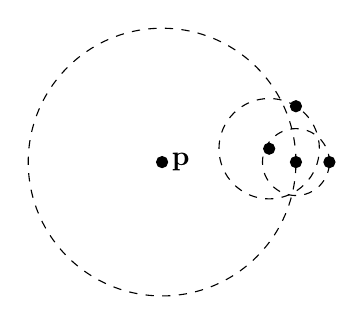
\begin{tikzpicture}[x=0.85cm,y=0.85cm]
\filldraw[black] (0,0) circle (2pt) node[anchor=west] {$\mathbf{p}$};
\draw[dashed] (0,0) circle (2);
\filldraw[black] (1.6,0.2) circle (2pt);
\filldraw[black] (2,0.834429) circle (2pt);
\draw[dashed] (1.6,0.2) circle (0.75);
\filldraw[black] (2,0) circle (2pt);
\filldraw[black] (2.5,0) circle (2pt);
\draw[dashed] (2,0) circle (0.5);
\end{tikzpicture}
\caption{Lorsque $k=2$, $\mathbf{p}$ est une valeur aberrante puisque sa densit\'e est plus faible que celle de ces voisins.}
\label{lofoutlier}
\end{figure}
\noindent L'algorithme LOF peut identifier les \textbf{observations aberrantes locales}, mais il n'est pas \'evident de choisir un seuil de densit\'e au-delà duquel un point est considéré comme une aberration. L'algorithme introduit aussi l'idée d'une \textbf{distance d'accessibillité}, ce qui améliore la stabilité des résultats au sein des groupes/régions: dans un $k-$voisinage local de $\mathbf{p}$, c'est tout simplement la distance maximale à ses $k$ voisins imm\'ediats; \`a l'ext\'erieur de cette région, c'est la distance actuelle de $\mathbf{p}$. 
\par \'A la figure \ref{reachability} (o\`u $k=3$), par exemple, les points $\mathbf{q}_1, \mathbf{q}_2, \mathbf{q}_3$ ont tous la même distance d'accessibilité de $\mathbf{p}$ car ce sont les 3 voisins imm\'ediats de $\mathbf{p}$, c'est-à-dire, 
$$
d_{\text{acc}}(\mathbf{p}, \mathbf{q}_1) 
= d_{\text{acc}}(\mathbf{p}, \mathbf{q}_2)
= d_{\text{acc}}(\mathbf{p}, \mathbf{q}_3)
= d(\mathbf{p}, \mathbf{q}_3)
.$$
Pour $\mathbf{q}_4$, en revanche, nous avons  
$d_{\text{acc}}(\mathbf{p}, \mathbf{q}_4)
= d(\mathbf{p}, \mathbf{q}_4)
$
puisque ce n'est pas un des 3 voisins imm\'ediats de $\mathbf{p}$.

\begin{figure}[H]
\hrule \vspace{0.4cm} \centering
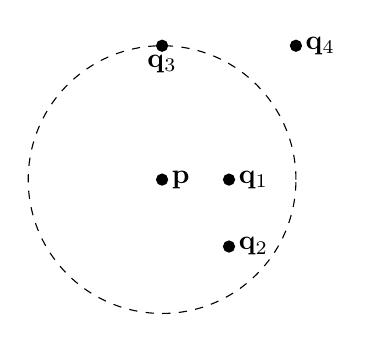
\begin{tikzpicture}[x=0.85cm,y=0.85cm]
\filldraw[black] (0,0) circle (2pt) node[anchor=west] {$\mathbf{p}$};
\filldraw[black] (1,0) circle (2pt) node[anchor=west] {$\mathbf{q}_1$};
\filldraw[black] (1,-1) circle (2pt) node[anchor=west] {$\mathbf{q}_2$};
\filldraw[black] (0,2) circle (2pt) node[anchor=north] {$\mathbf{q}_3$};
\filldraw[black] (2,2) circle (2pt) node[anchor=west] {$\mathbf{q}_4$};
\draw[dashed] (0,0) circle (2);
\end{tikzpicture}
\caption{Zone uniforme de distance d'accessibilit\'e autour de $\mathbf{p}$ pour $k=3$.}
\label{reachability}
\end{figure}
\newpage\noindent  

\subsubsection*{DBSCAN}
L'algorithme ``Density-Based Spatial Clustering of Applications with Noise'' (DBSCAN) a \'et\'e proposed en 1996 dans \cite{DBSCAN} (on en trouve un r\'esum\'e \`a la section 6.4.2 de \cite{A10}). Comme son nom l'indique, il s'agit d'un algorithme de regroupement ("clustering") reposant sur la densité qui regroupe les points voisins et identifie les points qui ne tombent pas dans les groupes comme  \textbf{anomalies}:
%Hierarchical DBSCAN (HDBSCAN) \cite{HDBSCAN} was introduced in 2013. It notably removes the problem of choosing the parameter for the radius of a neighbourhood by considering all possible radii. 
%Further documentation can be found at \cite{HDBSCAN_code}. 
 \begin{itemize}[noitemsep]
\item $\mathbf{p}$ est un \textbf{central} si au moins $m$ autres observations sont \`a une distance au plus $r$ de $\mathbf{p}$;
\item $\mathbf{q}$ est un \textbf{point frontière} s'il n'est pas lui-même un point central mais se trouve à une distance au plus $r$ d'un tel point, and 
\item $\mathbf{o}$ est une \textbf{anomalie} si ce n'est ni un point central ni un point frontière.
\end{itemize}

\begin{figure}[b]
\hrule \vspace{0.4cm}
\centering
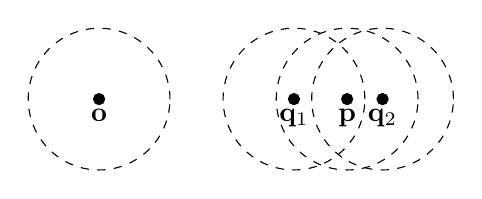
\begin{tikzpicture}[x=0.9cm,y=0.9cm]
\filldraw[black] (-3.5,0) circle (2pt) node[anchor=north] {$\mathbf{o}$};
\draw[dashed] (-3.5,0) circle (1);
\filldraw[black] (0,0) circle (2pt) node[anchor=north] {$\mathbf{p}$};
\draw[dashed] (0,0) circle (1);
\filldraw[black] (-0.75,0) circle (2pt) node[anchor=north] {$\mathbf{q}_1$};
\draw[dashed] (-0.75,0) circle (1);
\filldraw[black] (0.5,0) circle (2pt) node[anchor=north] {$\mathbf{q}_2$};
\draw[dashed] (0.5,0) circle (1);
\end{tikzpicture}
\caption{Avec $m=2$ et un rayon fixe $r$, $\mathbf{o}$ est une anomalie, $\mathbf{p}$ un point central, et $\mathbf{q}_1$ et $\mathbf{q}_2$ sont des points frontières.}
\label{DBSCANlabels}
\end{figure}
\noindent DBSCAN considère chaque point de l'ensemble de données individuellement. Si ce point est une anomalie, il est ajouté à une liste d'anomalie. Sinon, s'il s'agit d'un point central, son $r-$voisinage forme le point de d\'epart d'un nouveau groupe (``cluster''). Chaque point du voisinage est alors considéré à son tour, et les $r-$voisinages des autres points centraux contenus dans le voisinage sont ajoutés au groupe. \par Cette expansion se répète jusqu'à ce que tous les points aient été examinés. \`A ce stage, les points qui étaient auparavant considérés comme des points aberrants peuvent être mis à jour à mesure qu'ils deviennent des points frontaliers dans ce nouveau groupe. Ce processus se poursuit jusqu'à ce que chaque point ait été soit attribué à un groupe, soit étiqueté comme une valeur aberrante (cf.\@ l'Algorithme~\ref{dbscan} et la Figure~\ref{DBSCANlabels} pour plus de d\'etails).

Bien que la double utilisation de DBSCAN en tant qu'al\-go\-rith\-me de regroupement puisse sembler non pertinente dans le cadre de la détection des observations aberrantes, sa capacité à identifier avec succès les groupes naturels est cruciale car elle permet d'étiqueter les points qui subsistent comme des observations aberrantes.
\newl 
D'une part, le nombre de groupes n'a pas besoin d'être connu à l'avance (contrairement au  partitionnement en $k-$moyennes) et des groupes de forme arbitraire peuvent être détectés. \par Par ailleurs, seul le paramètre de la taille minimale des groupes ($m$) est requis. Ce dernier peut être défini de manière assez intuitive (ce qui n'est pas le cas pour les algorithmes partitionnement généraux): si les éléments de $D$ sont de dimension $n$, on choisit $m\geq n+1$ (plus la valleur de $m$ est grande, meilleure est l'identification du bruit). \begin{algorithm}[t]
\SetAlgorithmName{Algorithme}{}\SetAlgoLined
\textbf{Entr\'ees:} donn\'ees $D$,
distance $d$,
rayon de voisinage $r>0$,
taille maximale $m\in\mathbb{N}$ des groupes  
\\$\textit{Groupes} = \{\}$
\\$\textit{Anomalies} = \{\}$
\\\For{$\mathbf{p} \in D$}{
\If{$\mathbf{p} \in \textrm{Outliers} \cup \left( \cup_{C \in \textit{Clusters}} C \right)$}{
\textbf{continue}
}
D\'efinir $N(\mathbf{p}) = \{ \mathbf{q} \in D : d(\mathbf{p},\mathbf{q}) \leq r \}$
\\\If{$|N(\mathbf{p})| < m$}{
Ajouter $\mathbf{p}$ aux $\textit{Anomalies}$
\\\textbf{continue}
}
\Else{
$\textit{Groupe} = N(\mathbf{p})$
\\\For{$\mathbf{q} \in \text{Groupe} \setminus \{\mathbf{p}\}$}{
\If{$\mathbf{q} \in \textit{Anomalies}$}{
\'Eliminer $q$ des $\textit{Anomalies}$
}
\ElseIf{$\mathbf{q} \in \cup_{C \in \textit{Groupes}} C$}{
\textbf{continue}
}
D\'efinir $N(\mathbf{q}) = \{ q' \in D : d(q,q') \leq r \}$
\\\If{$|N(\mathbf{q})| \geq m$}{
$\text{Cluster} = \text{Cluster} \cup N(\mathbf{q})$
}
}
}
Ajouter $\textit{Groupe}$ \`a $\textit{Groupes}$
}
\textbf{Sortie:} liste des  \textit{anomalies}
\caption{DBSCAN}
\label{dbscan}
\end{algorithm}
\newl D'autre part, DBSCAN n'est pas un algorithme déterministe, car les points frontaliers peuvent être affectés à différents groupes selon l'ordre dans lequel les points centraux sont considérés (cela n'affecte toutefois pas son utilisation comme algorithme de détection des anomalies).
\par Dans des ensembles de haute dimension, la capacité de toute fonction de distance basée sur la distance euclidienne à distinguer les points proches et éloignés diminue en raison du \textbf{fl\'eau de la dimensionalit\'e}; et DBSCAN devient une m\'ethode de d\'efction inefficace (tout comme les autres algorithmes de partitionnement). \par Finalement, DBSCAN ne peut pas gérer les différences de densités locales car le rayon d'un$r-$voisinage est fixe; cela peut mener à des groupes plus éparses \'etant étiquetés comme observation aberrante, ou à ce que les observations aberrantes entourant un groupe plus dense \'etant incluses dans le groupe. Ce problème est surmonté dans HDBSCAN.

\subsubsection*{Forêt d'isolement}
Les approches discutées précédemment construisent d'abord des modèles de ce à quoi ressemblent les points normaux, puis identifient les points qui ne correspondent pas à ce modèle.
En revanche, l'algorithme de la forêt d'isolement \cite{A15} tente plutôt d'identifier explicitement les valeurs aberrantes en partant de l'hypothèse qu'il y a peu de valeurs aberrantes et que ces valeurs aberrantes ont des attributs très différents des points normaux. Cela permet d'utiliser des techniques d'échantillonnage, ce qui augmente la vitesse de traitement de l'algorithme tout en diminuant les besoins en mémoire.
\begin{figure}[b]
\hrule \vspace{0.4cm}\centering
\begin{tikzpicture}[x=0.58cm,y=0.58cm]
\filldraw[black] (0,0) circle (2pt);
\filldraw[black] (4,2) circle (2pt);
\filldraw[black] (4.5,-2) circle (2pt);
\filldraw[black] (5,1) circle (2pt);
\draw[dashed] (0,2) -- (0,-2);
\draw[dashed] (5,2) -- (5,-2);
\draw[dashed] (0,2) -- (5,2);
\draw[dashed] (0,-2) -- (5,-2);
\draw (2,2) -- (2,-2);
\draw (2,-1) -- (5,-1);
\draw (4.25,2) -- (4.25,-1);
\end{tikzpicture}
\caption{Une partition construite pendant la génération d'un arbre d'isolement.}
\label{isolationtree}
\end{figure}

L'algorithme de la forêt d'isolement tente d'isoler les points anormaux. Pour ce faire, on sélectionne un attribut de manière aléatoire, puis une valeur de séparation entre les valeurs minimale et maximale de cet attribut. De cette mani\`ere, on isole chaque observations dans sa propre partition.
\newl Ce partitionnement récursif produit un arbre binaire appelé \textbf{arbre d'isolement}. La racine de cet arbre est l'ensemble des données dans son intégralité; chaque nœud est un sous-ensemble des observations, et chaque branche correspond à l'une des partitions générées. Les feuilles représentent des ensembles simples contenant un seul point isolé. Chaque point se voit ensuite attribuer une note dérivée de la profondeur à laquelle sa partition isolée apparaît dans l'arbre (cf.\@ la  Figure~\ref{isolationtree} et l'Algorithme~\ref{iTree} pour plus de d\'etails). 
\par Comme les points qui se retrouvent moins profondément dans l'arbre sont plus faciles à séparer du reste, ce sont des \textbf{anomalies} probables. Seuls les points peu profonds présentent un intérêt; une fois que l'arbre atteint une hauteur donnée (la hauteur attendue d'un arbre binaire aléatoire, par exemple), la construction de l'arbre peut être arrêtée, ce qui réduit le coût de calcul. \par 
De plus, au lieu de construire un arbre à partir de l'ensemble des données, on peut construire un arbre à partir d'un sous-ensemble. L'emplacement de n'importe quel point dans ce plus petit arbre peut alors être estimé, ce qui permet d'économiser des ressources de calcul et de mémoire. Ces deux améliorations sont détaillées dans l'article original \cite{A15}. 
\newl Une fois qu'un certain nombre d'arbres d'isolement ont été générés de manière aléatoire (ce qu'on appelle une \textbf{forêt d'isolement}), un score peut être calculé pour chaque observation. Pour ce faire, on recherche son emplacement dans chaque arbre et on note la longueur du chemin nécessaire pour l'atteindre. La longueur moyenne du chemin est le score d\'esir\'e.
\newpage 
\begin{algorithm}[t]
\SetAlgorithmName{Algorithme}{}\SetAlgoLined
\textbf{\'Entr\'ees:} donn\'ees $D$ % , integer $e$ current tree height, integer $\ell$ max tree height
\\\If{$|D| \leq 1$}{ % $e \geq \ell$ \textbf{or} 
return $\{\}$
}
\Else{
Soit $\overline{A}$ la liste des variables de $D$
\\Choisir une variable  $A \in \overline{A}$ fa\c{c}on al\'eatoire
\\Choisir au hasard une valeur $s\in  [\min_{\mathbf{q} \in D} A(\mathbf{q}), \max_{\mathbf{q} \in D} A(\mathbf{q})]$
\\Return 
$\text{Node}\begin{cases}
\text{LeftChild} &= \text{iTree}(\{\mathbf{q} \in D : A(\mathbf{q}) \leq s\}) % , e+1, \ell\})
\\\text{RightChild} &= \text{iTree}(\{\mathbf{q} \in D : A(\mathbf{q}) > s\}) % , e+1, \ell\})
\\\text{NodeValue} &= D
\end{cases}$
\\ Répéter 2-9 avec $D=$LeftChild et $D=$RightChild
}
\textbf{Sortie:} arbre d'isolement binaire% of height $\leq \ell - e$ 
\caption{Arbre d'isolement: $\text{iTree}(D)$} % , e, \ell)$
\label{iTree}
\end{algorithm}

\noindent Il peut être souhaitable de construire un score d'anomalie normalisé, qui soit indépendant de la taille de l'ensemble de données.
Pour ce faire, on approxime la longueur de trajet prévue d'un point aléatoire dans un arbre d'isolation (c'est-à-dire un arbre binaire). Avec $n = |D|$, on peut montrer que la longueur moyenne est 
$$
c(n) 
= 2 H(n-1) - \frac{2(n-1)}{n},
$$
o\`u $H(n-1)$ est le $(n-1)^{\text{e}}$ nombre harmonique, dont la valeur approximative est $\ln(n-1) + 0.577$;
on utilise $c(n)$ afin de normaliser le score d'anomalie $a(\mathbf{p})$, $\mathbf{p} \in D$, which is given by
$$
\log_2 a(\mathbf{p})
= -\frac{\text{hauteur moyenne de $\mathbf{p}$ dans $\text{iTrees}(D)$}}{c(n)}.
$$
Ainsi défini, $a(\mathbf{p})\in [0,1]$. Si $a(\mathbf{p}) \approx 1$, on consid\`ere que $\mathbf{p}$ est une \textbf{anomalie}; si $a(\mathbf{p}) \leq 0.5$, on consid\`ere que $\mathbf{p}$ est un point r\'egulier; si tous les points reçoivent un score pr\`es de $0.5$, cela suggère qu'il n'y a pas d'anomalie dans l'ensemble de donn\'ees.
\newl Les forêts d'isolement demandent  tr\`es peu de resources de temps et de mémoire; elles peuvent traiter des données de grande dimension, et n'ont pas besoin d observations  étiquetées, ce qui est un \'enorme avantage, mais le score d'anomalie attribué à un point donné peut avoir une variance élevée apr\`es plusieurs r\'ep\'etitions de l'algorithme. Les auteurs de \cite{EIF} proposent des solutions \`a ce problème.
\begin{center}\rule{0.5\linewidth}{.4pt}\end{center}
En général, les m\'ethodes reposant sur la densit\'e sont plus efficaces que celles reposant sur la distance lorsqu'un ensemble de données contient des structures ayant des caractéristiques diverses, mais moins efficaces lorsque les structures sont de densités comparables avec les observations aberrantes \cite{JZ}.
\begin{algorithm}[h]
\SetAlgorithmName{Algorithme}{}\SetAlgoLined
\textbf{\'Entr\'ees:} donn\'ees $D$, nombre d'arbres d'isolement $t$ % , integer $n$ subsampling size
\\\textit{For\^et} = \{\}
% \\Set max tree height 
% $\ell = \lceil \log_2(n) \rceil$
\\\For{$i=1$ to $t$}{
% \\$D' \leftarrow sample(D, n)$
\textit{Arbre} = $\text{iTree}(D)$ % , 0, \ell)$
\\Ajouter \textit{Arbre} \`a \textit{For\^et}
}
\For{$\mathbf{p} \in D$}{
$\textit{HauteurChemin} = \{\}$
\\\For{\textit{Arbre} in \textit{For\^et}}{
% \\\If{$\{\mathbf{p}\}$ not a node of Tree}{
% }
% \\\Else{
Calculer la hauteur $\ell$ du noeud $\{\mathbf{p}\}$ dans l'Arbre
\\Ajouter $\ell$ \`a $\textit{HauteurChemin}$
}
$\textit{HauteurCheminMoy} = \frac{\sum_{\ell \in \textit{HauteurChemin}} \ell}{t}$
\\D\'efinir $a(\mathbf{p}) = 2^{- \frac{\textit{HauteurCheminMoy}}{c(|D|)}} $
}
\textbf{Sortie:} score d'anomalie $a(\mathbf{p}) \in [0,1]$ pour chaque observation $\mathbf{p} \in D$
\caption{For\^et d'isolement}
\label{iForest}
\end{algorithm}